% Created by tikzDevice version 0.8.1 on 2016-01-28 18:51:29
% !TEX encoding = UTF-8 Unicode
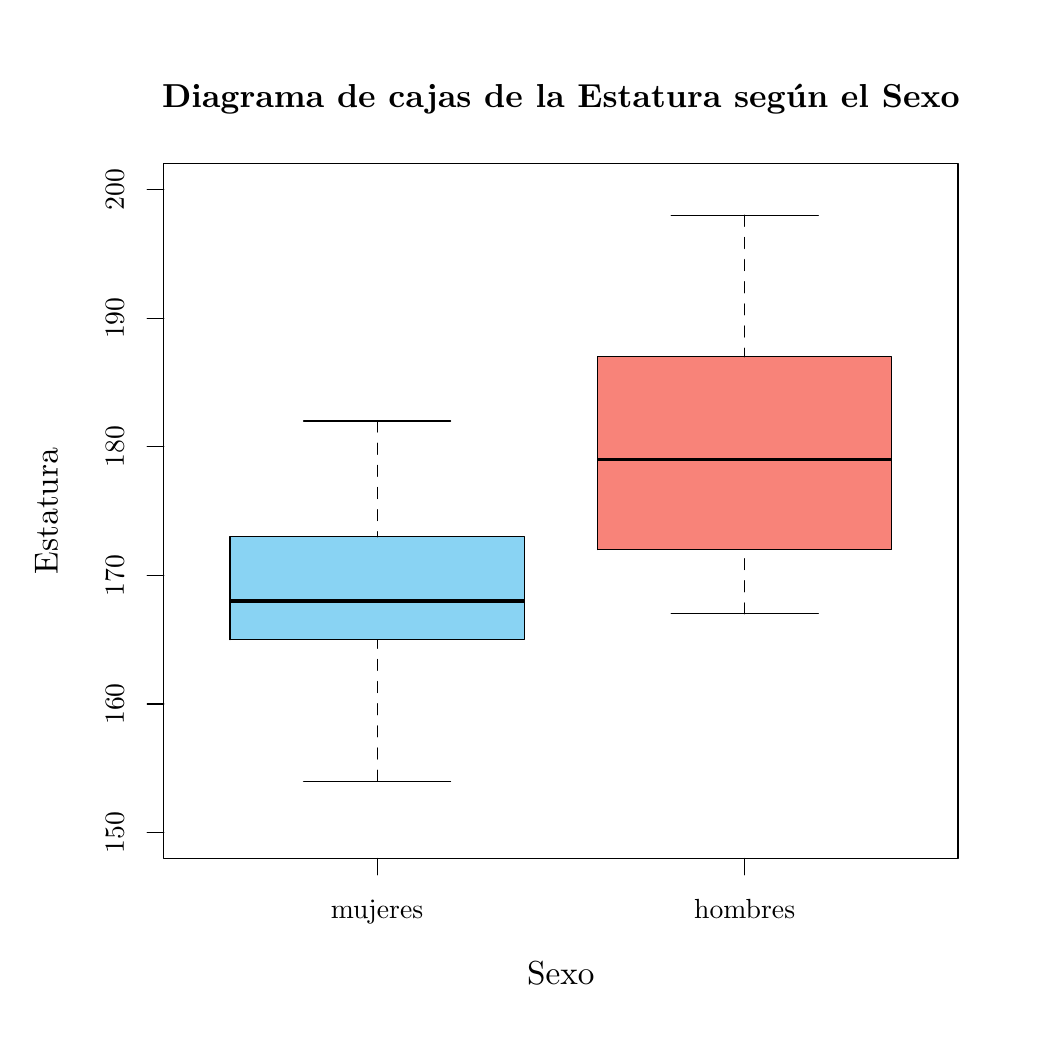
\begin{tikzpicture}[x=1pt,y=1pt]
\definecolor{fillColor}{RGB}{255,255,255}
\path[use as bounding box,fill=fillColor,fill opacity=0.00] (0,0) rectangle (361.35,361.35);
\begin{scope}
\path[clip] ( 49.20, 61.20) rectangle (336.15,312.15);
\definecolor{fillColor}{RGB}{137,211,243}

\path[fill=fillColor] ( 73.11,140.20) --
	(179.39,140.20) --
	(179.39,177.38) --
	( 73.11,177.38) --
	cycle;
\definecolor{drawColor}{RGB}{0,0,0}

\path[draw=drawColor,line width= 1.2pt,line join=round] ( 73.11,154.14) -- (179.39,154.14);

\path[draw=drawColor,line width= 0.4pt,dash pattern=on 4pt off 4pt ,line join=round,line cap=round] (126.25, 89.08) -- (126.25,140.20);

\path[draw=drawColor,line width= 0.4pt,dash pattern=on 4pt off 4pt ,line join=round,line cap=round] (126.25,219.21) -- (126.25,177.38);

\path[draw=drawColor,line width= 0.4pt,line join=round,line cap=round] ( 99.68, 89.08) -- (152.82, 89.08);

\path[draw=drawColor,line width= 0.4pt,line join=round,line cap=round] ( 99.68,219.21) -- (152.82,219.21);

\path[draw=drawColor,line width= 0.4pt,line join=round,line cap=round] ( 73.11,140.20) --
	(179.39,140.20) --
	(179.39,177.38) --
	( 73.11,177.38) --
	( 73.11,140.20);
\definecolor{fillColor}{RGB}{248,131,121}

\path[fill=fillColor] (205.96,172.73) --
	(312.24,172.73) --
	(312.24,242.44) --
	(205.96,242.44) --
	cycle;

\path[draw=drawColor,line width= 1.2pt,line join=round] (205.96,205.26) -- (312.24,205.26);

\path[draw=drawColor,line width= 0.4pt,dash pattern=on 4pt off 4pt ,line join=round,line cap=round] (259.10,149.50) -- (259.10,172.73);

\path[draw=drawColor,line width= 0.4pt,dash pattern=on 4pt off 4pt ,line join=round,line cap=round] (259.10,293.56) -- (259.10,242.44);

\path[draw=drawColor,line width= 0.4pt,line join=round,line cap=round] (232.53,149.50) -- (285.67,149.50);

\path[draw=drawColor,line width= 0.4pt,line join=round,line cap=round] (232.53,293.56) -- (285.67,293.56);

\path[draw=drawColor,line width= 0.4pt,line join=round,line cap=round] (205.96,172.73) --
	(312.24,172.73) --
	(312.24,242.44) --
	(205.96,242.44) --
	(205.96,172.73);
\end{scope}
\begin{scope}
\path[clip] (  0.00,  0.00) rectangle (361.35,361.35);
\definecolor{drawColor}{RGB}{0,0,0}

\path[draw=drawColor,line width= 0.4pt,line join=round,line cap=round] (126.25, 61.20) -- (259.10, 61.20);

\path[draw=drawColor,line width= 0.4pt,line join=round,line cap=round] (126.25, 61.20) -- (126.25, 55.20);

\path[draw=drawColor,line width= 0.4pt,line join=round,line cap=round] (259.10, 61.20) -- (259.10, 55.20);

\node[text=drawColor,anchor=base,inner sep=0pt, outer sep=0pt, scale=  1.00] at (126.25, 39.60) {mujeres};

\node[text=drawColor,anchor=base,inner sep=0pt, outer sep=0pt, scale=  1.00] at (259.10, 39.60) {hombres};

\path[draw=drawColor,line width= 0.4pt,line join=round,line cap=round] ( 49.20, 70.49) -- ( 49.20,302.86);

\path[draw=drawColor,line width= 0.4pt,line join=round,line cap=round] ( 49.20, 70.49) -- ( 43.20, 70.49);

\path[draw=drawColor,line width= 0.4pt,line join=round,line cap=round] ( 49.20,116.97) -- ( 43.20,116.97);

\path[draw=drawColor,line width= 0.4pt,line join=round,line cap=round] ( 49.20,163.44) -- ( 43.20,163.44);

\path[draw=drawColor,line width= 0.4pt,line join=round,line cap=round] ( 49.20,209.91) -- ( 43.20,209.91);

\path[draw=drawColor,line width= 0.4pt,line join=round,line cap=round] ( 49.20,256.38) -- ( 43.20,256.38);

\path[draw=drawColor,line width= 0.4pt,line join=round,line cap=round] ( 49.20,302.86) -- ( 43.20,302.86);

\node[text=drawColor,rotate= 90.00,anchor=base,inner sep=0pt, outer sep=0pt, scale=  1.00] at ( 34.80, 70.49) {150};

\node[text=drawColor,rotate= 90.00,anchor=base,inner sep=0pt, outer sep=0pt, scale=  1.00] at ( 34.80,116.97) {160};

\node[text=drawColor,rotate= 90.00,anchor=base,inner sep=0pt, outer sep=0pt, scale=  1.00] at ( 34.80,163.44) {170};

\node[text=drawColor,rotate= 90.00,anchor=base,inner sep=0pt, outer sep=0pt, scale=  1.00] at ( 34.80,209.91) {180};

\node[text=drawColor,rotate= 90.00,anchor=base,inner sep=0pt, outer sep=0pt, scale=  1.00] at ( 34.80,256.38) {190};

\node[text=drawColor,rotate= 90.00,anchor=base,inner sep=0pt, outer sep=0pt, scale=  1.00] at ( 34.80,302.86) {200};
\end{scope}
\begin{scope}
\path[clip] (  0.00,  0.00) rectangle (361.35,361.35);
\definecolor{drawColor}{RGB}{0,0,0}

\node[text=drawColor,anchor=base,inner sep=0pt, outer sep=0pt, scale=  1.20] at (192.68,332.61) {\bfseries Diagrama de cajas de la Estatura según el Sexo};

\node[text=drawColor,anchor=base,inner sep=0pt, outer sep=0pt, scale=  1.20] at (192.68, 15.60) {Sexo};

\node[text=drawColor,rotate= 90.00,anchor=base,inner sep=0pt, outer sep=0pt, scale=  1.20] at ( 10.80,186.68) {Estatura};
\end{scope}
\begin{scope}
\path[clip] (  0.00,  0.00) rectangle (361.35,361.35);
\definecolor{drawColor}{RGB}{0,0,0}

\path[draw=drawColor,line width= 0.4pt,line join=round,line cap=round] ( 49.20, 61.20) --
	(336.15, 61.20) --
	(336.15,312.15) --
	( 49.20,312.15) --
	( 49.20, 61.20);
\end{scope}
\end{tikzpicture}
